%!TEX root = ../thesis.tex
%*******************************************************************************
%****************************** Second Chapter *********************************
%*******************************************************************************

\chapter{The spatiotemporal expression of RdDM components and small RNA landscapes in the germline of \textit{Arabidopsis thaliana}}

\ifpdf
    \graphicspath{{Chapter2/Figs/Raster/}{Chapter2/Figs/PDF/}{Chapter2/Figs/}}
\else
    \graphicspath{{Chapter2/Figs/Vector/}{Chapter2/Figs/}}
\fi


\section{Abstract}


%\begin{figure}[htbp!] 
%\centering    
%
\includegraphics[width=1.0\textwidth]{minion}
%\caption[Minion]{This is just a long figure caption for the minion in Despicable Me from Pixar}
%\label{fig:minion}
%\end{figure}

\section{Introduction}

\clearpage



\section{NRPD1 is expressed in the tapetum, microspores but not in meiocytes}

Since RNA polymerase IV and V preferentially associate with methylated RNA, RdDM is thought of as a self-reinforcing pathway. Therefore the observation that there are few perfect matching 24nt sRNAs in MetGenes in Arabisopsis meiocytes, it was hypothesised that the Pol IV dependent pathway is quiescent and that the sRNAs directing DNA methyaltion at MetGenes are produced from HyperTE loci in the tapetum that target HyperTE and MetGene methylation in the meiocyte \citep{RN199,RN187}. To confirm this expression pattern, pNRPD1::NRPD1-eGFP and pNRPE1::NRPE1-eGFP fluorescent reporter lines (of the largest subunits of RNA Polymerase IV and V respectively\citep{RN33}) were constructed by dr Jincheng Long.

The columella in the root tip of Arabidopsis is hypermetylated in the CHH context \citep{RN261}, the root tip was imaged to screen and select the best lines selected for further imaging (Figure\ref{fig:Pol4_5_roots}).

\begin{figure}[htbp!] 
\centering    
    \includegraphics[width=1\textwidth]{Chapter2/Figs/Figure3_Pol4_anther_gynecium.pdf}
\caption{\textbf{NRPD1 is expressed in the tapetum, microspore and gynoecium.}}
\label{fig:Pol4_anther}
\captionsetup{font=small}
    \caption*{NRPD1 expression in meiocyte stage anthers in the tapetum and surrounding somatic cells(first row, third column (GFP, green, white arrows), and expression in microspores (second row third column, white arrows). NRPD1 is also expressed in both the germ and somatic cells of the meiocyte stage gynoecium (third row (GFP, green)). Scale bar 10 $\mu$m.}
\end{figure}

Meiocytes are surrounded by the tapetum - a somatic tissue layer of nurse cells with cytoplasmic connections to meiocytes through plasmodesmata. As expected, NRDP1 expression was confined to the tapetal layer and surrounding somatic anther tissue in meiocyte stage anthers (Figure \ref{fig:Pol4_anther}). Once meiocytes undergo meiosis, the plasmodesmatal connection to the tapetum ceases and the meiocytes are surrounded by callose cell walls. At the microspore stage, the germline cells express NRPD1 (Figure \ref{fig:Pol4_anther} second row, \ref{fig:Pol4_germ} first and second rows). NRPD1 was also expected to be expressed strongly in the maternal reproductive tissue \citep{RN165} which was confirmed in several independent reporter lines (Figure \ref{fig:Pol4_anther}, row three).

Following a further two cell divisions, the bicellular and tricellular pollen grains are produced, neither of which express NRPD1 (Figure \ref{fig:Pol4_germ}, rows 3 and 4). However, it must be added that the expression levels of the best NRPD1 reporter lines were a lot lower and more diffuse than the expression of NRPE1 or CLSY3 reporter lines (Figures \ref{fig:CLSY3_anther}, \ref{fig:Pol4_5_roots}). Further, expression in germline tissues wasn't consistent even in lines that exhibited strong root signal (Figure \ref{fig:Pol4_germ}, Figure \ref{fig:Pol4_germ_no_expression}). As these results are from screening 37 independent transformants from the same transformation event, it would be worth constructing new transformants perhaps with a stronger fluorescent reporter (such as tdTomato) to corroborate these results, and confidently confirm whether NRPD1 is expressed in the pollen. 


\begin{figure}[htbp!] 
\centering    
    \includegraphics[width=0.8\textwidth]{Chapter2/Figs/Figure4_Pol4_germline.pdf}
\caption{\textbf{NRPD1 is expressed in microspores, but its expression is absent in pollen}}
\label{fig:Pol4_germ}
\captionsetup{font=small}
    \caption*{NRPD1 expression early and late microsproes (first and second rows, third column (GFP, green, white arrows), and expression in microspores (second row third column, white arrows). NRPD1 however us not expressed in bicellular or tricellular pollen (third and fourth rows (DAPI, blue GFP, green). Scale bar 10 $\mu$m.}
\end{figure}

\section{NRPE1 is expressed in both somatic and germline tissues in \textit{Arabidopsis} anthers}

According to methylation and 24nt sRNA datasets,  PolV-dependent pathway of RdDM be active in the somatic tapetal layer and meiocytes, but it wasn't clear what happens after meiosis in microspores and pollen. As before, strong nuclear signal was confirmed in the root tip (Figure \ref{fig:Pol4_5_roots}).  NRPE1 is strongly expressed in meiocytes, tapetum and in the surrounding somatic tissues of the meiocyte stage anther (Figure \ref{fig:Pol5_germ}, first row). This expression also persists into both soma and germline of microspore stage anthers and the female meiocyte stage gynoecium (Figure \ref{fig:Pol5_germ} second and third rows respectively), indicating that the RNA polymerase V pathway of RdDM is active in both somatic and germline cells of the anther. As we know RdDM is highly active in maternal reproductive tissue, the expression of NRPE1 was confirmed in this tissue as well (Figure \ref{fig:Pol5_germ}, third row).

\begin{figure}[htbp!] 
\centering    
    \includegraphics[width=1\textwidth]{Chapter2/Figs/Figure5_Pol5_germline.pdf}
\caption{\textbf{NRPE1 is expressed in the tapetum, meiocyte, microspores and gynoecium}}
\label{fig:Pol5_germ}
\captionsetup{font=small}
    \caption*{NRPE1 expression in meiocyte stage anthers in the tapetum, meiocyte and surrounding somatic cells(first row, third column (GFP, green, white arrows), and expression in microspores (second row third column, white arrows). NRPE1 is also expressed in both the germ and somatic cells of the meiocyte stage gynoecium (third row (GFP, green)). Scale bar 10 $\mu$m.}
\end{figure}


\section{CLSY3 is expressed in the tapetum of meiocyte stage anthers and in the gynoecium}

CLSY3 chromatin remodeller drives sRNA production in the tapetum \citep{RN187} by recruiting Pol IV to discrete loci (including HyperTEs)\citep{RN23}. In accordance with this, the expression on CLSY3 in meiocyte stage anthers is largely restricted to the tapetum (Figure \ref{fig:CLSY3_anther} first row), with diminished expression in the tapetum after meiosis (Figure \ref{fig:CLSY3_anther} second row). CLSY3 is also required for expression of abundant 24nt sRNA in the ovules and therefore it is strongly expressed in the gynoecium and surrounding somatic tissues (Figure \ref{fig:CLSY3_anther}, third row).

\begin{figure}[htbp!] 
\centering    
    \includegraphics[width=0.8\textwidth]{Chapter2/Figs/Figure1_CLSY3_anther_gynecium.pdf}
\caption{\textbf{CLSY3 is expressed in the tapetum of meiocyte stage anthers and in the gynoecium}}
\label{fig:CLSY3_anther}
\captionsetup{font=small}
    \caption*{CLSY3 is strongly expressed in the nucleus of meiocyte stage tapetal cells (first row (Venus, yellow)), which then diminishes in the senescing tapetum after meiosis in the microspore stage(second row, Venus (yellow)). CLSY3 is also expressed in both the germ and somatic cells of the meiocyte stage gynoecium (third row (Venus, yellow)). Scale bar 10 $\mu$m.}
\end{figure}

However, following meiosis, CLSY3 is not expressed in microspore, bicellular or tricellular pollen stages (Figure \ref{fig:CLSY3_germ}) highlighting the restricted spatiotemporal expression of CLSY3 to produce 24nt sRNAs at HyperTEs and drive methylation of these loci, as well as MetGene loci in the meiocyte. Although endogenous sRNA production is active in the microspore (Figure \ref{fig:Pol4_germ}), and potentially in pollen, CLSY3 does not play a significant role in shaping the 24nt sRNA and CHH methylation landscapes during these stages of development.

\begin{figure}[htbp!] 
\centering    
    \includegraphics[width=0.8\textwidth]{Chapter2/Figs/Figure2_CLSY3_germline.pdf}
\caption{\textbf{CLSY3 is not expressed in the male germline cells}}
\label{fig:CLSY3_germ}
\captionsetup{font=small}
    \caption*{DAPI stained microspore, bicellular or tricellular pollen (second column (DAPI, blue). CLSY3 signal not detected in any germline cells (third row (Venus, yellow). Scale bar 10 $\mu$m}
\end{figure}

Together, these results demonstrate: NRPD1 and therefore RNA Polymerase IV is active in the somatic tapetal cells in meiocyte stage anthers but not in meiocytes, and in the germline cells within microspore stage anthers; NRPE1 and therefore RNA Polymerase V is active in both somatic and germline cells in meiocyte and microspore stage anthers. The ambiguous results of NRPD1 expression in the microspores suggests that constructing new fluorescent reporter lines with a stronger fluorescent reporter (such as tdTomato) would be needed to corroborate these results and confirm NRPD1 expression in the pollen.


\section{HyperTE sRNAs decline proportionally post-meiosis, despite elevated proportional dominance of 24nt sRNAs in sperm cells}

To dissect the dynamics of the sRNA landscape in the germline, sRNA sequencing libraries were constructed for microspores, sperm cells, and sperm nuclei (2 replicates each). These were then compared to meiocyte and tapetum sRNA libraries \citep{RN187}, as well as to somatic sRNA sequencing libraries \citep{RN262,RN263,RN264}. 

All three somatic tissues sampled had a strong 21nt and 24nt peak (Figure \ref{fig:sRNA_sizes}A). However, in the germline, except for microspores, the dominant sRNA length was 24nt, with sperm cells and sperm nuclei exhibiting the highest proportional levels of 24nt sRNA (Figure \ref{fig:sRNA_sizes}B).

\begin{figure}[htbp!] 
\centering    
    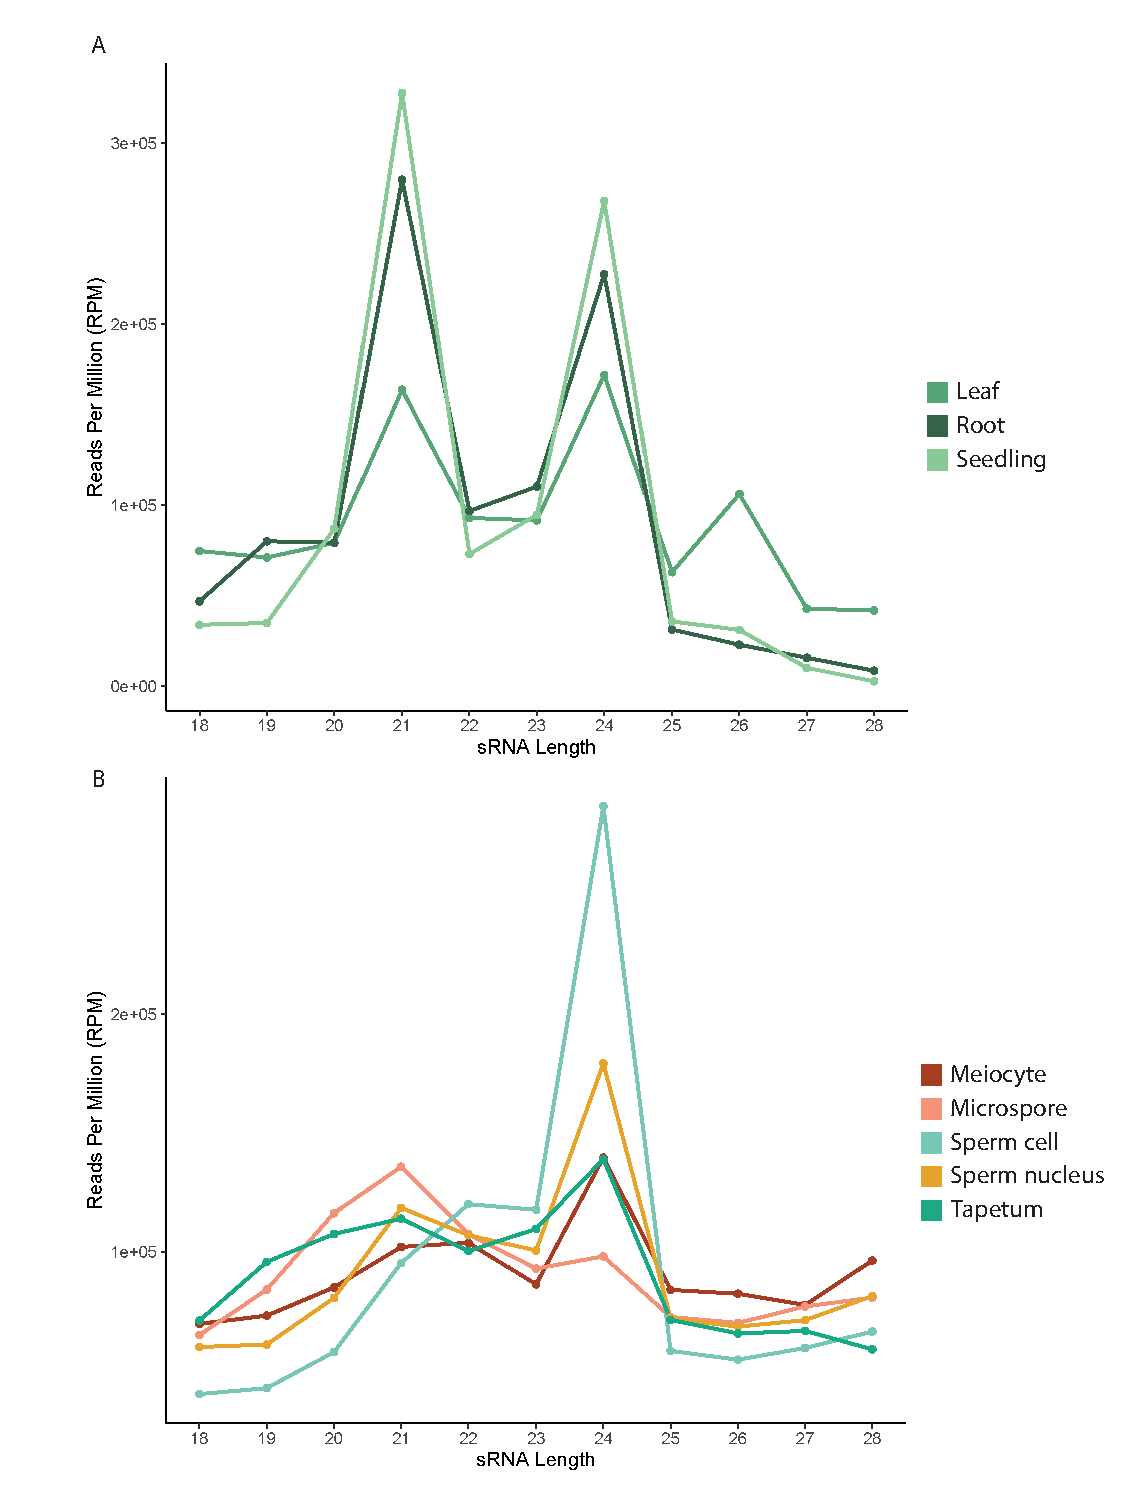
\includegraphics[width=0.8\textwidth]{Chapter2/Figs/Figure6_sRNA_sizes.pdf}
\caption{\textbf{In germline tissues, the dominant sRNA length is 24nt}}
\label{fig:sRNA_sizes}
\captionsetup{font=small}
    \caption*{(A) The size distribution of sRNAs in leaf, root and seedling. X axis: sRNA lengths, Y axis: reads per million (RPM) (B) The size distribution of sRNAs in meiocyte, microspore, sperm cell, sperm nucleus and tapetum. X axis: sRNA lengths, Y axis: reads per million (RPM)}
\end{figure}

When examining genomic features to capture a snapshot of 24nt sRNA distribution in germline tissues, it has been previously shown that HyperTEs dominate the 24nt sRNA landscape in meiocytes \citep{RN187}. However, the proportion of 24nt sRNAs within HyperTE regions gradually declines through cell divisions following meiosis, from meiocytes to sperm cells, suggesting that endogenous HyperTE sRNA production does not continue or ceases in the germline cells after meiosis and the closure of the plasmodesmatal connections to microspores. (Figure \ref{fig:sRNA_pie}A). 

In sperm cells, TE regions become the dominant source of 24nt sRNAs, mirroring the pattern observed in somatic tissues (Figure \ref{fig:sRNA_pie}B). In somatic tissues a large portion of these canonical RdDM loci are known to be associated with CLSY1 and CLSY2 \citep{RN23}. However, in the pollen, neither CLSY1 nor CLSY2 were strongly expressed (Figure \ref{fig:clsy1_2_pollen} suggesting (provided there's endogenous sRNA production in the pollen), these clusters are not strongly associated with the expression of any protein from the CLSY family.

\begin{figure}[htbp!] 
\centering    
    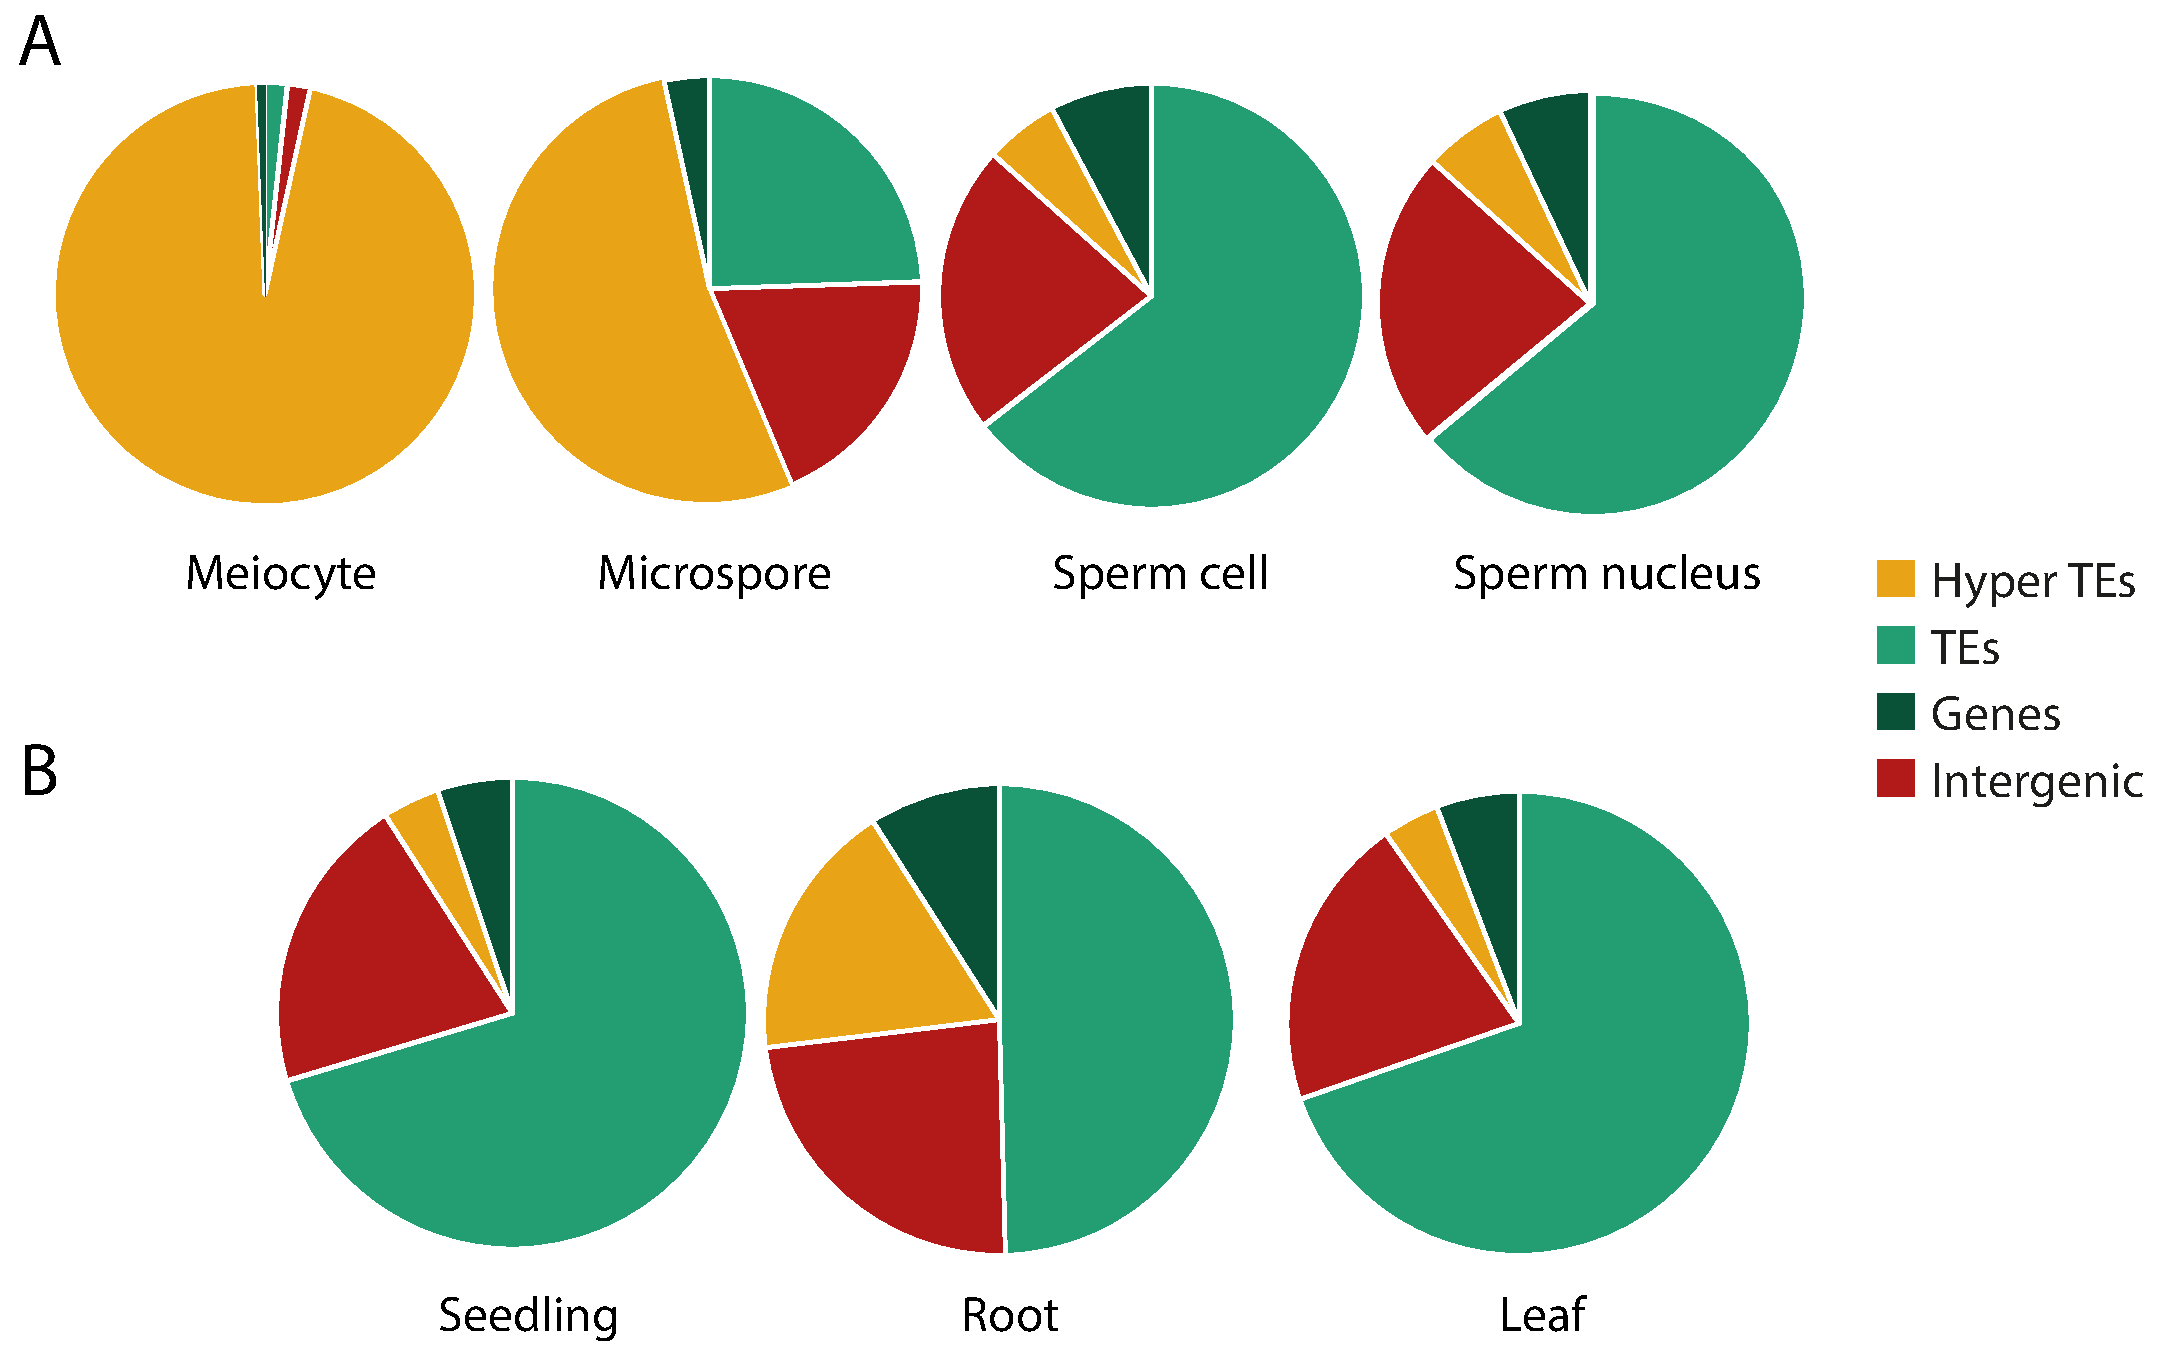
\includegraphics[width=0.8\textwidth]{Chapter2/Figs/Figure7_Pie_charts.pdf}
\caption{\textbf{HyperTE derived 24nt sRNAs decline in proportional abundance after meiosis and throughout pollen development}}
\label{fig:sRNA_pie}
\captionsetup{font=small}
    \caption*{Pie chart showing the proportional mapping of 24nt sRNAs to genomic features of interest: HyperTEs, TEs, Genes, MetGenes and intergenic regions in (A) germline tissue (meiocyte, microspore, sperm cell and sperm nucleus) and (B) somatic tissue (seedling, root and leaf).}
\end{figure}

\section{Sperm Cell sRNA Clusters Are Uncoupled From CLSY-Dependent Loci}

Examining the expression levels of germline-associated CLSY3-dependent loci, HyperTEs, and somatic tissue-associated CLSY1/2-dependent loci, along with canonical RdDM (cRdDM) loci, we can first conclude that, as expected, CLSY1/2-dependent and cRdDM loci exhibit the highest overall abundance of sRNAs in somatic tissues (leaf, seedling, and root). In contrast, most cRdDM loci do not generate sRNAs in the meiocyte, tapetum, or microspore. Interestingly, the sperm cell and sperm nucleus appear to represent an intermediate stage, where sRNA production at cRdDM loci is reactivated though not to the same extent as in somatic tissues (Figures \ref{fig:hm_CLSY3_CLSY1}B,D, \ref{fig:boxplot-MCMS}).

Conversely, in CLSY3-dependent and HyperTE loci, we observe an opposite pattern: 24nt sRNA abundance is highest in the meiocyte, tapetum, and microspore (though somewhat reduced in the microspore at certain loci), while somatic tissues exhibit lower sRNA levels. The sperm cell and sperm nucleus again show intermediate sRNA abundance. Pollen, in particular, displays higher overall levels of 24nt sRNAs from these loci, suggesting they are primarily produced in the vegetative cell. Notably, a subset of HyperTE loci continues to produce sRNAs even in somatic tissues (Figures \ref{fig:hm_CLSY3_CLSY1}A-C, \ref{fig:boxplot-MCMS}).

Since the heatmaps show normalised levels of sRNA against total sRNA levels in each tissue, it must be ensured that these patterns are comparable. To achieve this, 24nt sRNA levels in the cRdDM loci were also normalized against 21nt miRNA levels, as these are assumed to remain constant across cell types. This approach yielded comparable sRNA levels across the tested tissues, validating the observed relative differences in sRNA patterns (Figure \ref{fig:miRNA_norm}).

\begin{figure}[htbp!] 
\centering    
    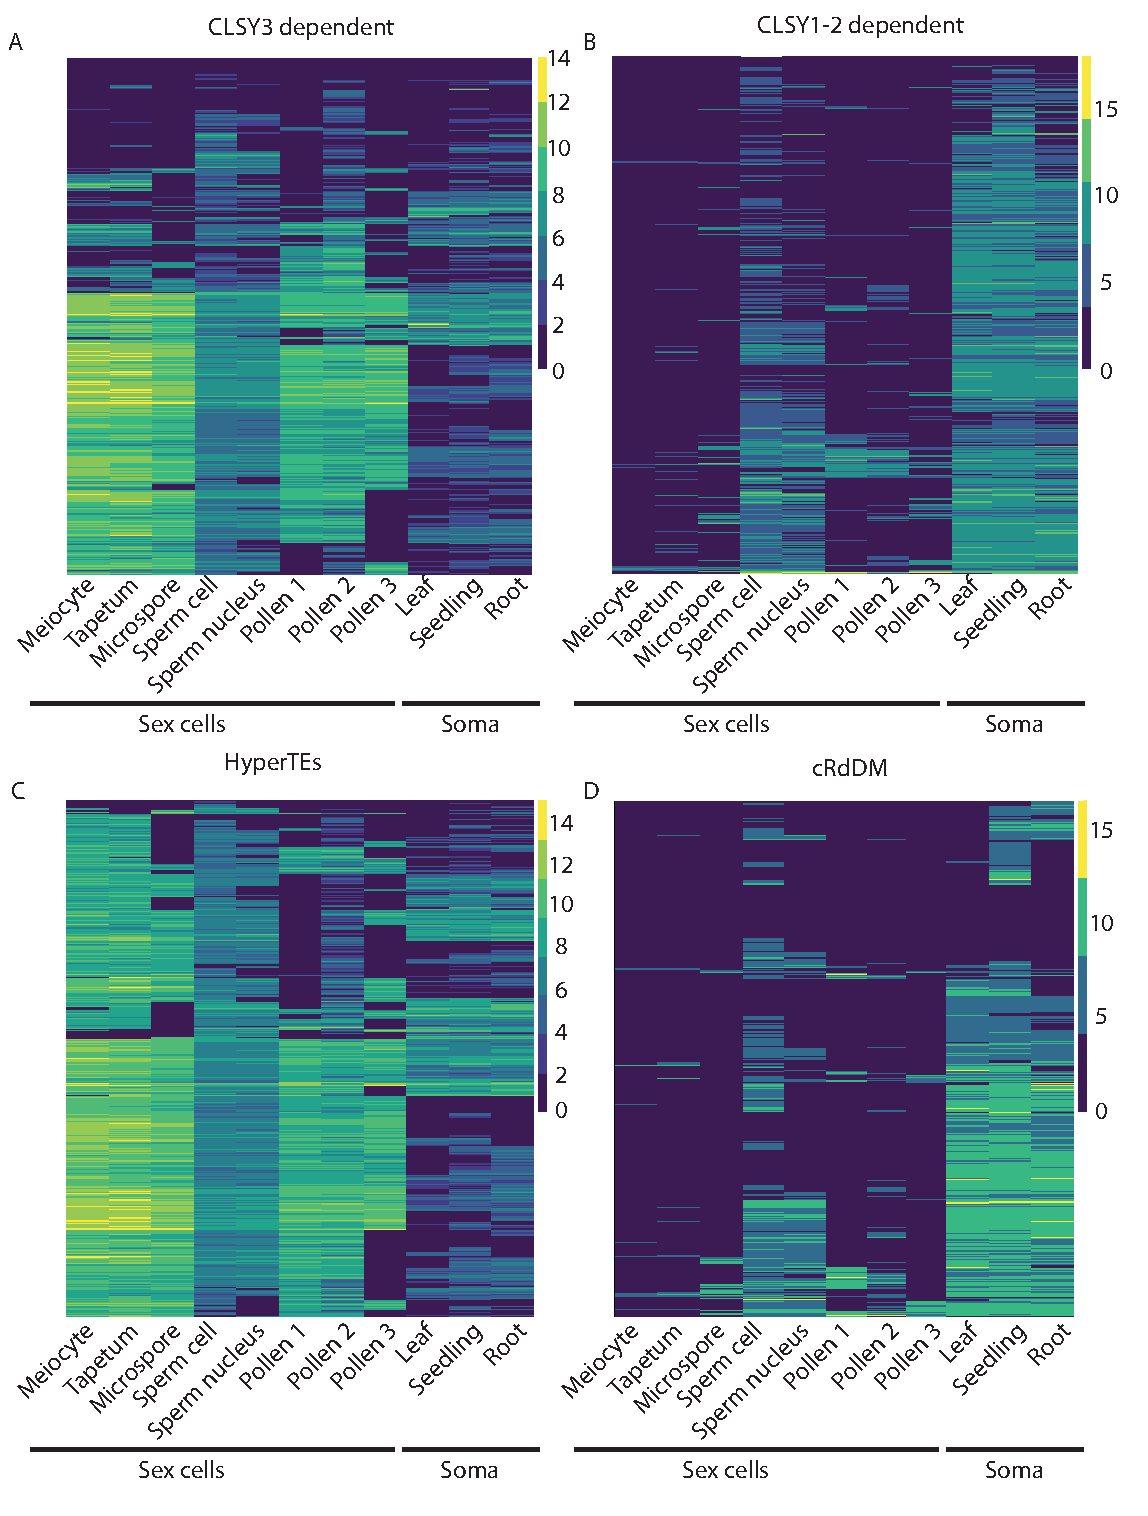
\includegraphics[width=0.8\textwidth]{Chapter2/Figs/Figure8_Heatmaps_CLSY3_CLSY1_2vs_cRdDMs_HyperTEs.pdf}
\caption{\textbf{CLSY3-dependent loci and HyperTEs generate abundant sRNAs in meiocytes and tapetum, as well as in microspores and sperm cells, though to a lesser degree. CLSY1\&2-dependent loci and canonical RdDM loci primarily produce abundant sRNAs in somatic tissues, with intermediate levels in sperm cells.}}
\label{fig:hm_CLSY3_CLSY1}
\captionsetup{font=small}
    \caption*{Heatmaps showing the 24nt sRNA RPKM levels of (A) CLSY3 dependent, (B) CLSY1\&2 dependent, (C) HyperTEs and (D) cRdDM loci in different germline (meiocyte, tapetum, sperm cell, sperm nucleus, pollen) and somatic tissues (leaf, seedling, root). Scale bar shows RPKM values.}
\end{figure}

To further understand the sRNA landscape in sperm and microspore, the sRNA profiles were compared pairwise to somatic tissues as well as other germline tissues, namely the meiocyte. Genome wide, 24nt sRNA abundance in 24nt clusters correlate weakly between the meiocyte and microspore (Figure \ref{fig:MSSVMC_scatters}A), but less so than between tapetum and meiocyte (Figure \ref{fig:scatter_SC_chromatin}A). This correlation is then further reduced between the meiocyte and sperm, indicating that global 24nt sRNA profiles are indeed vastly different between these cell types (Figure \ref{fig:MSSVMC_scatters}B).

Additionally, when comparing sperm cell-specific sRNA clusters between the meiocyte and sperm, and highlighting key genomic features, we clearly see that a significant subset of sperm-specific clusters producing sRNAs overlap with HyperTEs. These clusters have correspondingly high sRNA abundance in the meiocyte, with relatively lower abundance in the sperm cell (Figure \ref{fig:MSSVMC_scatters}B). In contrast, loci with low RPKM values in the meiocyte but high in sperm include a mixture of canonical RdDM loci and other sperm-specific loci that do not overlap with either HyperTEs or cRdDMs.

Similarly, highlighting CLSY-dependent loci in the same dataset (Figure \ref{fig:clsysingle_cRdDM_scatters}B) yields results consistent with those in Figure \ref{fig:MSSVMC_scatters}B. In Figure \ref{fig:clsysingle_cRdDM_scatters}B loci with abundant sRNAs in the meiocyte overlap CLSY3-dependent loci. Surprisingly, loci that produce sRNAs in sperm distinctly from the meiocyte do not exclusively overlap CLSY1 and CLSY2 dependent loci as would be expected in somatic tissues.Instead, many of these loci do not overlap with any CLSY-dependent loci. These findings underline the hypothesis that sperm cells exhibit a distinct sRNA profile compared to both earlier germline cells and somatic tissues.

\section{Distinct Chromatin and DNA Methylation Patterns in Sperm-Specific sRNA Loci}

Next, examining whether loci that produce abundant sRNAs in sperm compared to the seedling have different chromatin states, (based on H3K9me2 as an indicator of euchromatin or heterochromatin), we find that a subset of loci (n = 568) generating more small RNAs in sperm than in the seedling are predominantly heterochromatic (Figure \ref{fig:MSSVMC_scatters}C, red box). As expected, sperm cell-specific clusters show a strong correlation between the sperm cell and sperm nucleus (Figure \ref{fig:MSSVMC_scatters}D). Furthermore, loci synthesising the most abundant sRNA in both sperm cell and sperm nucleus tend to be heterochromatic.

\begin{figure}[htbp!] 
\centering    
    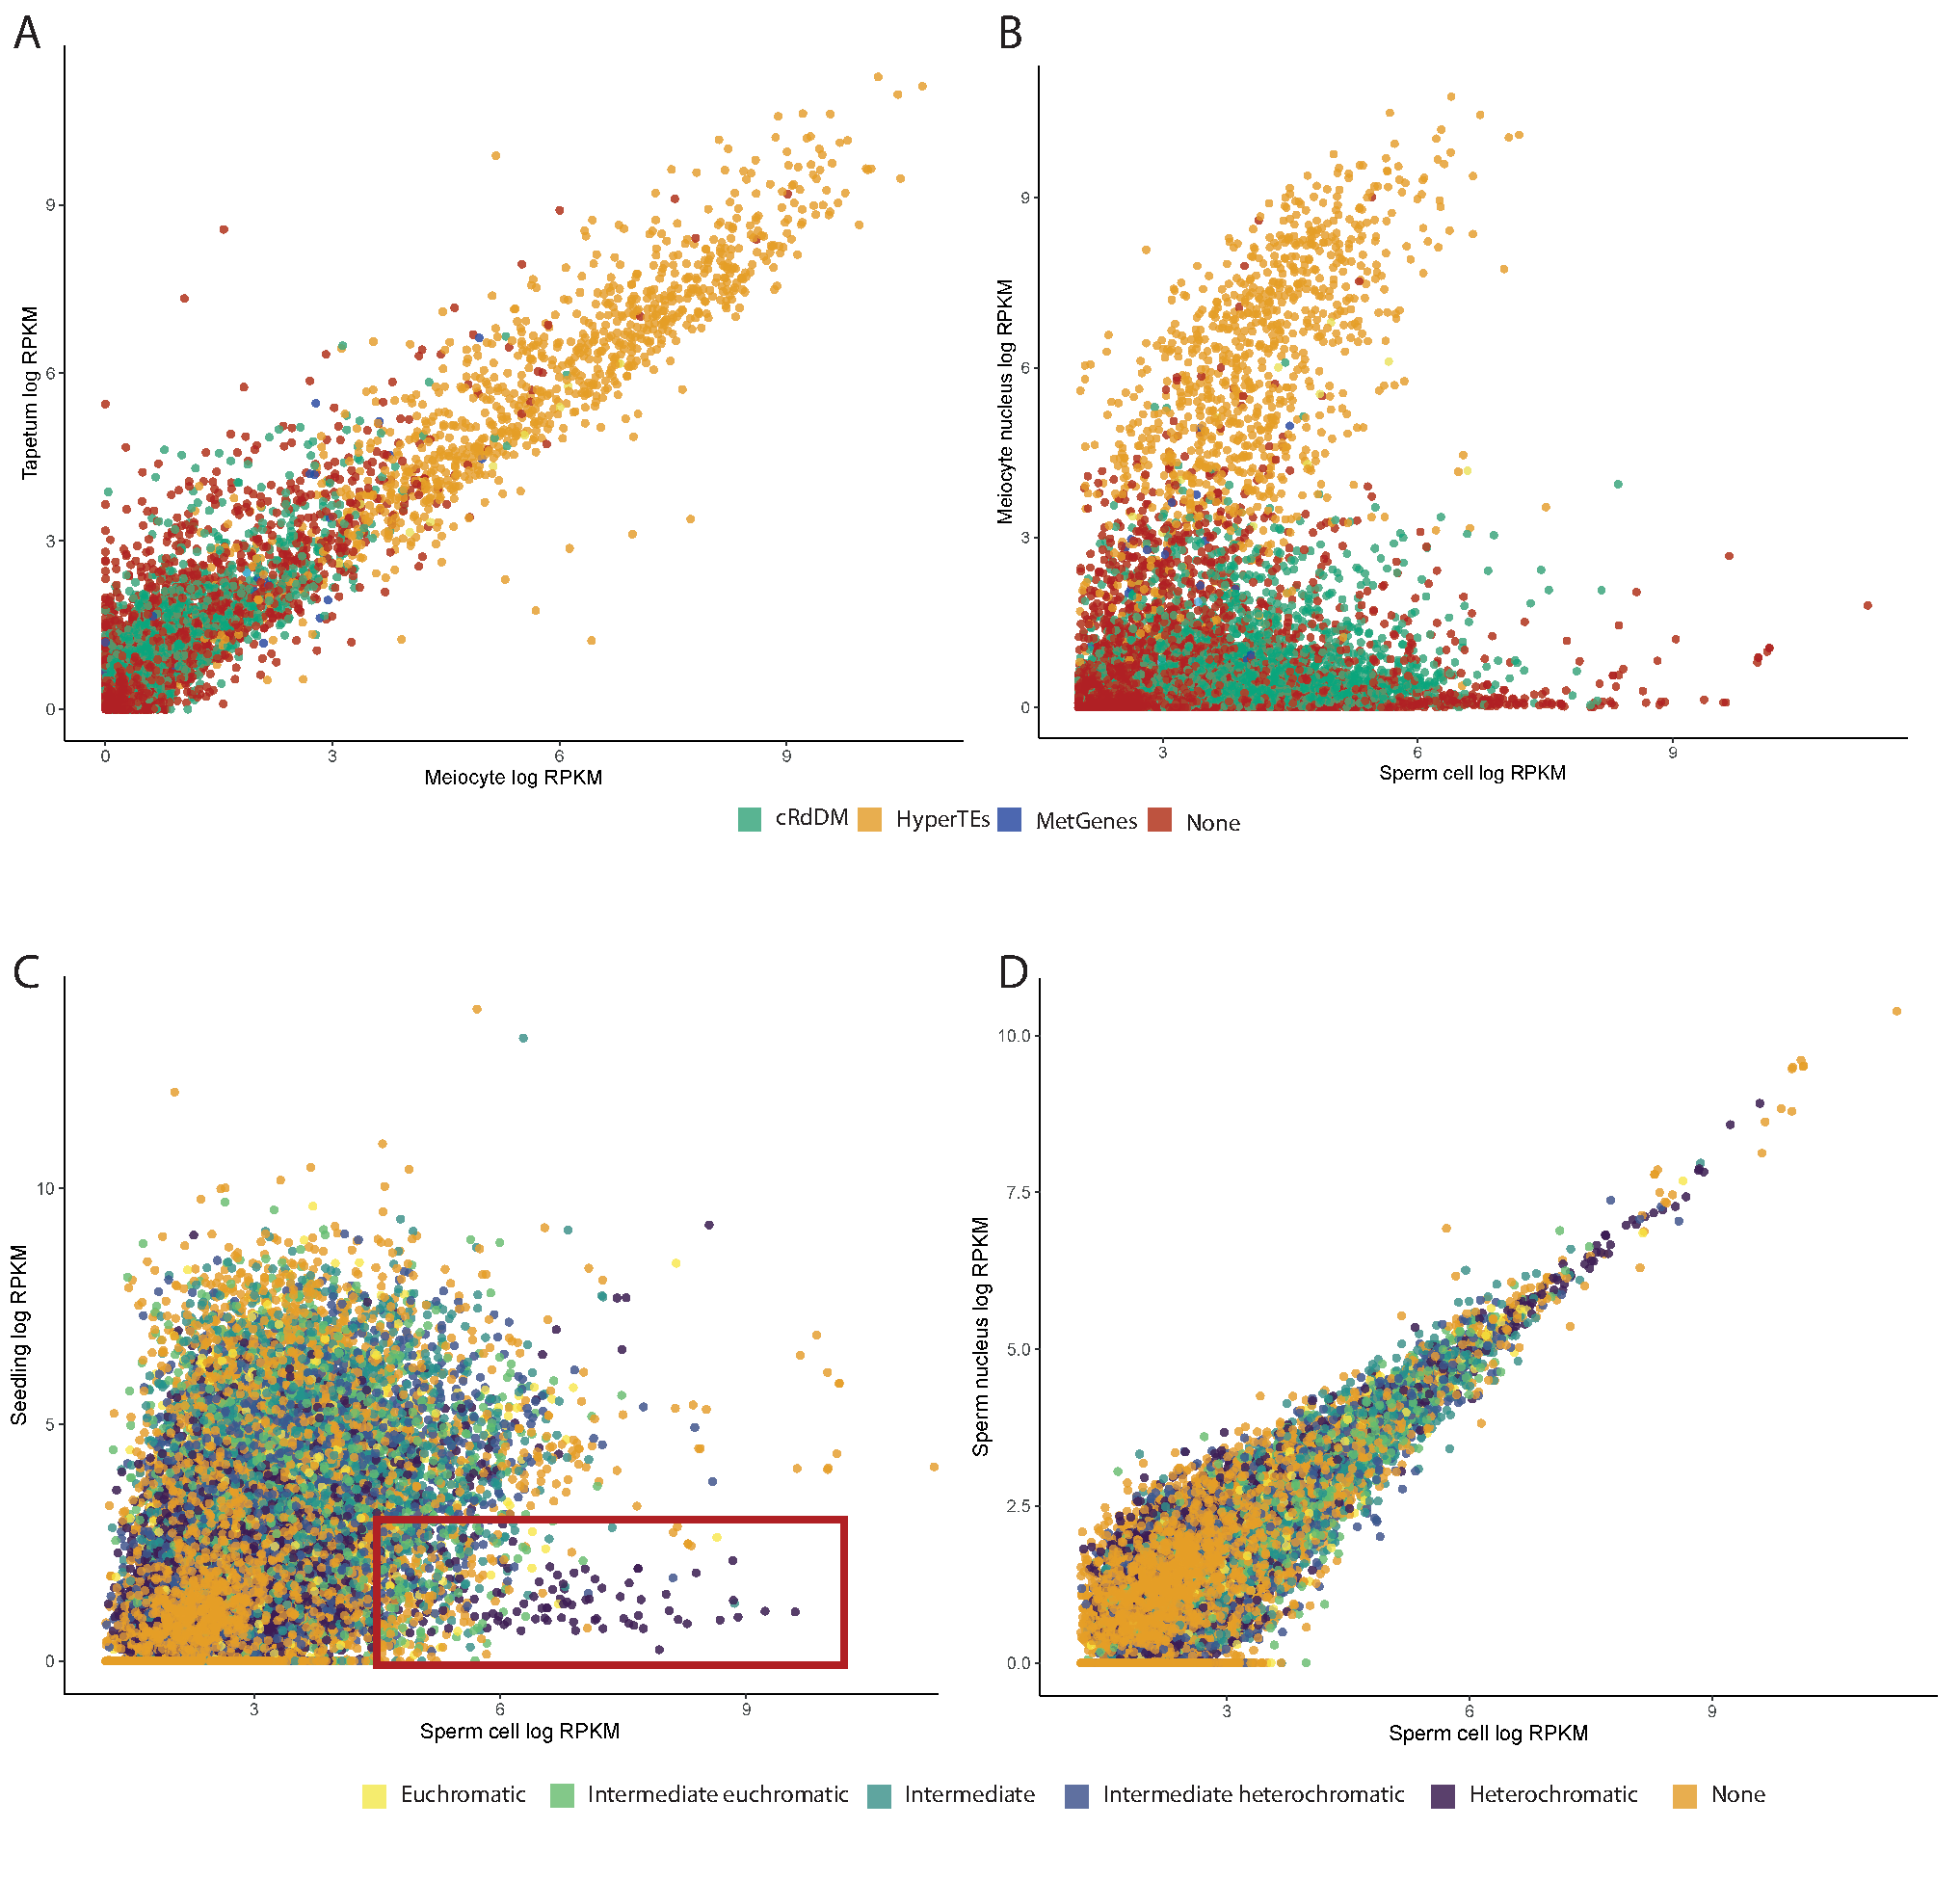
\includegraphics[width=1\textwidth]{Chapter2/Figs/Figure9_Scatterplots_HyperTEs_chromatin_SC.pdf}
\caption{\textbf{HyperTEs produce highly abundant 24nt sRNAs specifically in the meiocyte and tapetum which tapers off in the sperm cell. Loci with highly abundant 24nt sRNAs specifically in the sperm cell tend to be more heterochromatic.}}
\label{fig:scatter_SC_chromatin}
\captionsetup{font=small}
    \caption*{Correlations between 24nt sRNA abundance and the indicated cell types, highlighting (A-B) genomic features of interest and (C-D) chromatin structure. (C) Sperm cell specific heterochromatic cluster highlighed with red box. }
\end{figure}

It is crucial to investigate whether the heterochromatic sperm-specific n568 subcluster has a specific methylation pattern distinct from the whole set. We can conclude that generally, methylation in the sperm-specific sRNA clusters is consistently high, intermediate, and low in the CG CHG and CHH context throughout germline development respectively (Figure \ref{fig:SC_hetero_clusters}, dark green bars). In contrast, the n568 subcluster exhibits generally lower methylation levels compared to the full set (Figure \ref{fig:SC_hetero_clusters}, light green bars). However, when examining methylation patterns in other tissues, it becomes clear that this pattern is not exclusive to the sperm cell.

\begin{figure}[htbp!] 
\centering    
    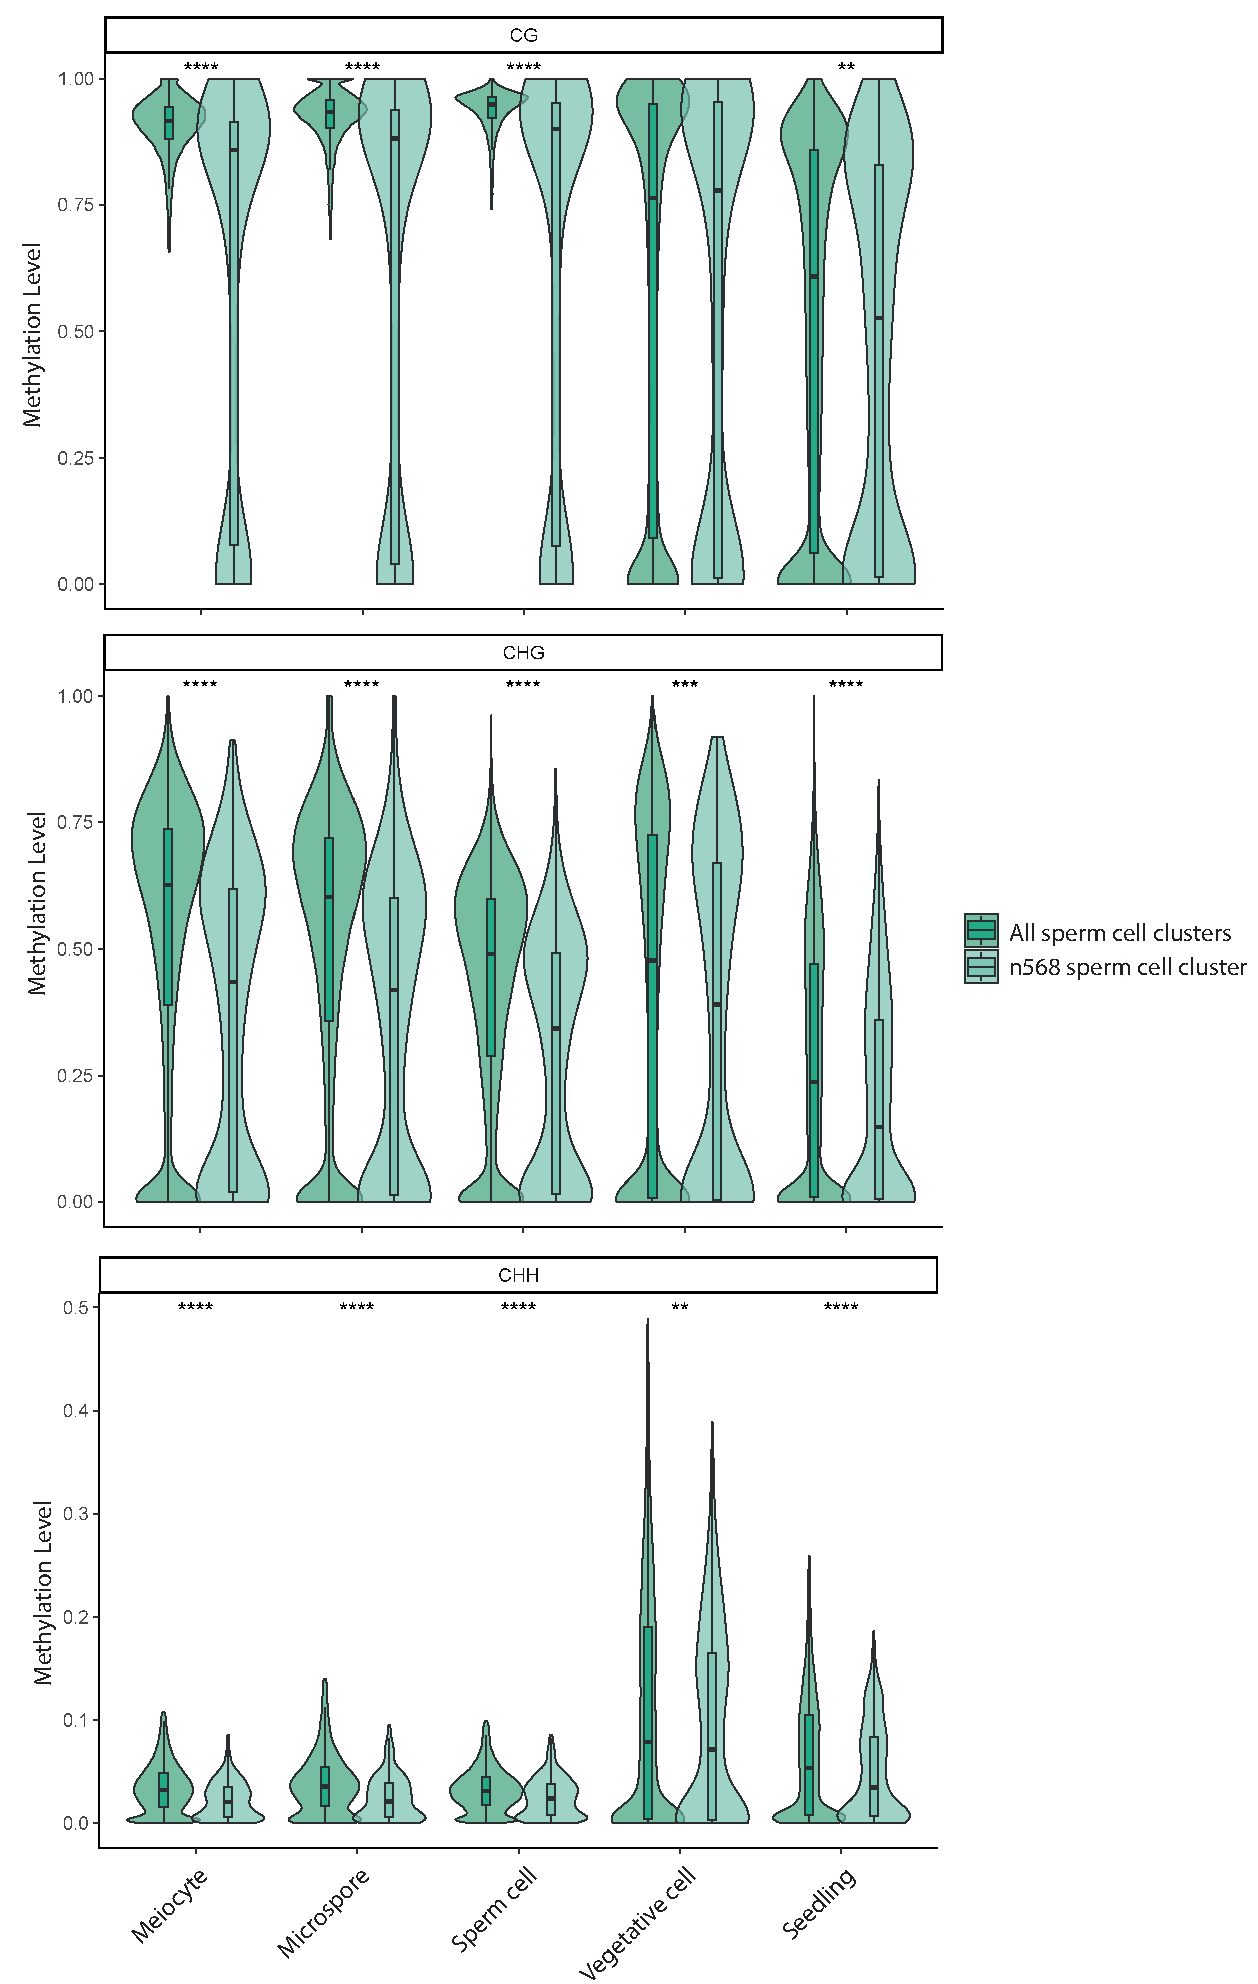
\includegraphics[width=1\textwidth]{Chapter2/Figs/Figure10_SC_hetero_clusters_methylation.pdf}
\caption{\textbf{Sperm-specific heterochromatic loci exhibit significantly lower overall methylation levels compared to the entire sperm dataset}}
\label{fig:SC_hetero_clusters}
\captionsetup{font=small}
    \caption*{CG, CHG and CHH methylation levels of all sperm clusters (dark green) and the heterochromatic 568 loci subset (light green). ***: p-value < 0.001, **: p-value < 0.01,*: p-value < 0.05}
\end{figure}

\section{A subset of MetGenes produce 24nt sRNAs and gain CHH methylation specifically in the sperm cell}

In contrast to other sex cells, about 20\% of MetGenes generate 24nt sRNAs in the sperm cell, with a subset producing sRNAs exclusively in sperm (Figure \ref{fig:hm_metgene_reactivated}, clusters 1 and 2, Figure \ref{fig:boxplot-SCPL}B). Since previous work has identified that MetGenes produce no perfect matching sRNAs in the meiocyte and tapetum\citep{RN187}, it is likely that the clusters which produce sRNAs in meiocyte and tapetum are either at HyperTE/MetGenes boundaries, or are HyperTE derived. However, the majority of sRNA producing MetGenes in the sperm cell and sperm nucleus do not overlap the same loci (Figure \ref{fig:hm_metgene_reactivated}, clusters 1 and 2: sperm specific reactivation, cluster 3: HyperTE/boundary derived meiocyte and tapetum specific clusters). Furthermore, the subset of loci that produce sRNAs uniquely in the sperm cell and sperm nucleus are not enriched in CLSY dependent loci (only 5 are broadly CLSY dependent out of 53 sperm specific reactivated MetGenes).

\begin{figure}[htbp!] 
\centering
    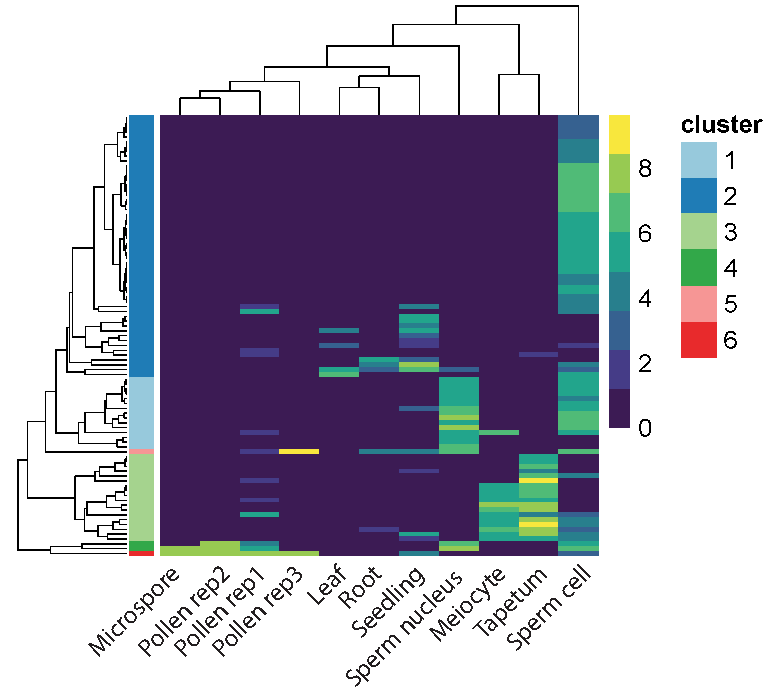
\includegraphics[width=0.8\textwidth]{Chapter2/Figs/Figure11_Reactivated_MetGenes_heatmap.pdf}
\caption{\textbf{Approximately 20\% of MetGenes produce sRNAs in the sperm}}
\label{fig:hm_metgene_reactivated}
\captionsetup{font=small}
    \caption*{Clusters 1,2: sperm specific sRNA production. Cluster 3: HyperTE/MetGene boundary derived meiocyte and tapetum specific clusters}
\end{figure}

Next, it was important to determine whether the increased sRNA production actually leads to increased DNA methylation in the sperm cell. Overall, the sperm cell-specific MetGenes exhibited higher CG and CHG methylation compared to the full set in meiocytes and microspores (Figure \ref{fig:boxplot_MetGene_methylation}A,B,D,E), and higher methylation in the CHG context in sperm. Interestingly, the only tissue where this subset showed higher CHH methylation was in the sperm cell, suggesting that renewed sRNA production at these loci also drives methylation in the sperm cell (Figure \ref{fig:boxplot_MetGene_methylation}C,F).

\begin{figure}[htbp!] 
\centering    
    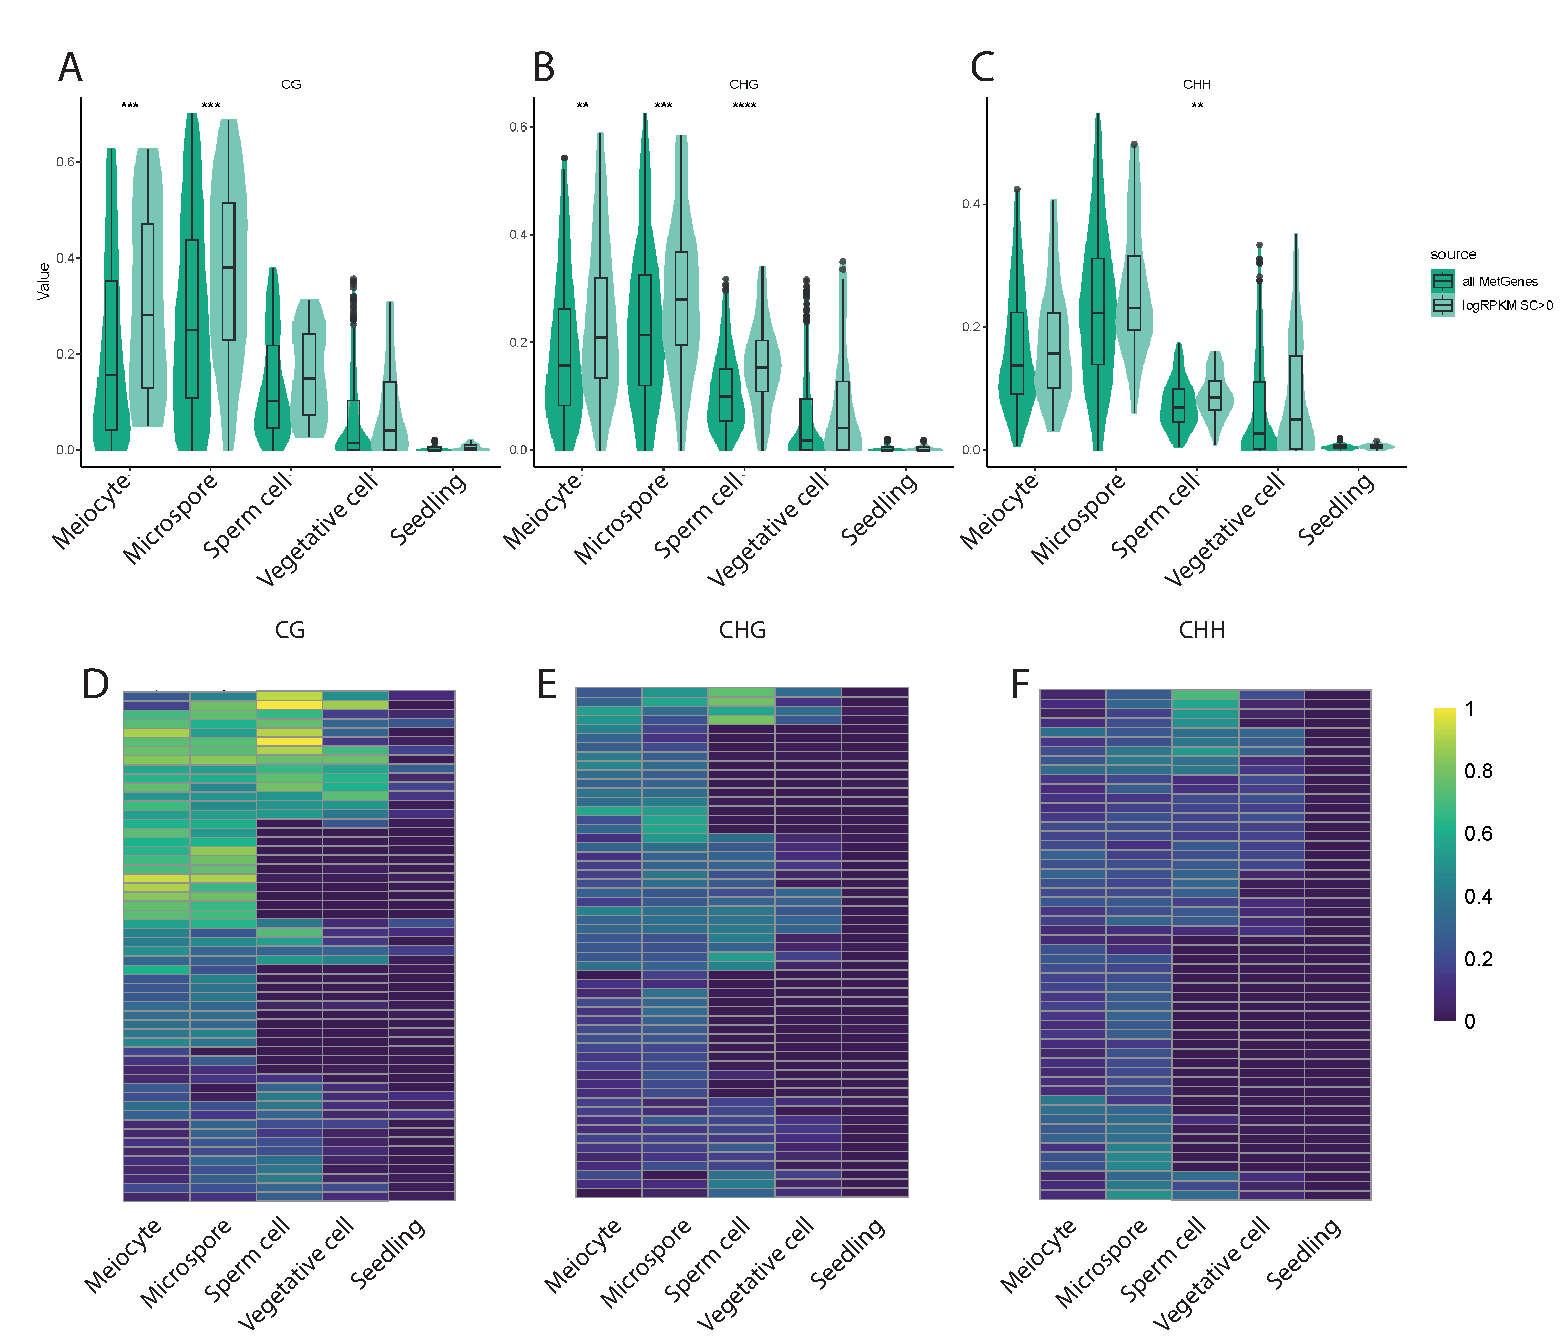
\includegraphics[width=1\textwidth]{Chapter2/Figs/Figure12_Reactivated_MetGenes_methylation.pdf}
\caption{\textbf{The reactivated MetGenes gain CHH methylation in the sperm cell.}}
\label{fig:boxplot_MetGene_methylation}
\captionsetup{font=small}
    \caption*{(Box plots of CG (A), CHG (B) and CHH (C) methylation of all MetGenes compared to the reactivated subset, in germline and somatic tissues. Heatmaps of the CG (D) CHG (E) and CHH (F) methylation MetGenes that produce sRNAs in the sperm cell. ***: p-value < 0.001, **: p-value < 0.01,*: p-value < 0.05}
\end{figure}

\section{ATGP2N TEs produce highly abundant 24nt sRNAs in sperm cells, the sperm nucleus, and pollen.}

As previously mentioned, after meiosis, HyperTE-derived sRNAs cease to be the dominant source of 24nt sRNAs in the sperm cell. Therefore it is important to analyse the landscape of 24nt sRNAs from sperm clusters overlapping TEs (Figure \ref{fig:TE_families}A). This revealed a cluster of TE families conserved across pollen, sperm cells, and sperm nuclei, which produce uniquely abundant sRNAs (Figure \ref{fig:TE_families}A, cluster 8, n=24). Within this subset, approximately 90\% of transposons belong to the LTR/Gypsy superfamily, and about 70\% are from the ATGP2 and ATGP2N families. Of these, about 40\% overlap CLSY3/4 dependent loci specifically.

\begin{figure}[htbp!] 
\centering    
    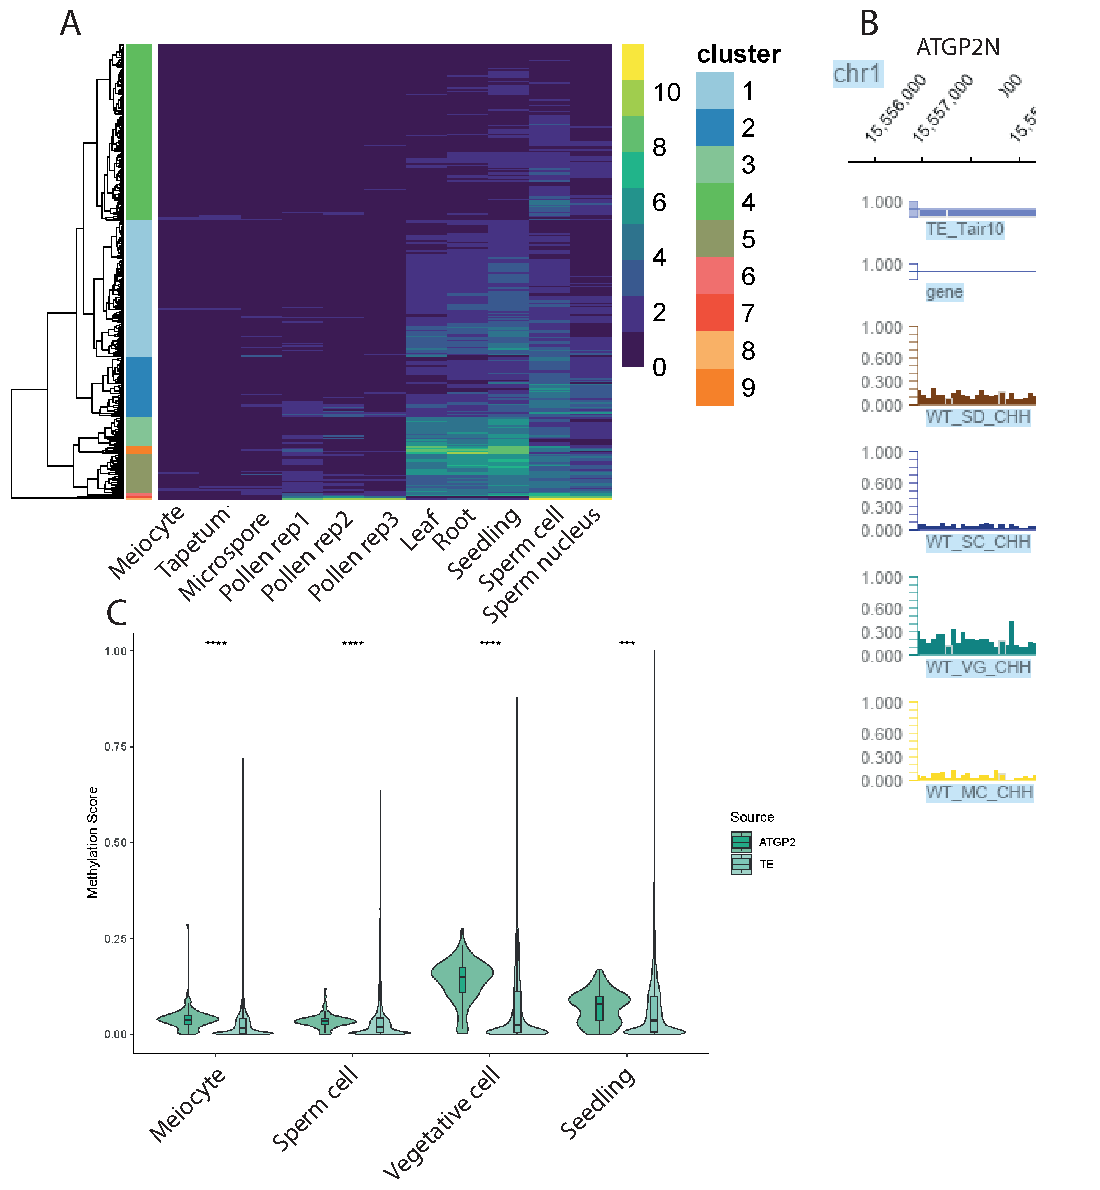
\includegraphics[width=0.8\textwidth]{Chapter2/Figs/Figure13_TE_families_heatmap.pdf}
\caption{\textbf{ATGP2N TEs produce highly abundant 24nt sRNAs in the sperm cell, sperm nucleus and pollen}}
\label{fig:TE_families}
\captionsetup{font=small}
    \caption*{(A) Heatmap showing the 24nt sRNA production of TE families in germline and somatic tissues. Cluster 9 contains the ATGP2N families.}
\end{figure}

Notably, another LTR/Gypsy transposon ATGP1 has been reported to be a direct target of RdDM in meiocytes, targeted by sRNAs produced in the tapetum, and gaining release from repression in RdDM defective mutants\citep{RN187}, specifically in the male germline.

ATGP2N has previously been reported to gain chromatin accessibility and be transcriptionally upregulated in \textit{met1} mutants. In this study ATGP2N was part of a subset of TEs that gained chromatin accessibility and increased in transcription as well as an increase in the production of 21nt sRNAs in the inflorescences of \textit{met1} mutants. The other groups gained accessibility but had no change in transcription or sRNA production, one already being highly expressed in wild type plants, and the other remaining repressed with respect to transcription and sRNA production even with increased chromatin accessibility\citep{RN184}. Though CHH methylation of TEs in the germline and somatic tissues seemed generally low, the ATGP2N family had slightly increased CHH methylation in all tissues, most notably for this study, in the vegetative cell (Figure \ref{fig:TE_methylation}B and C).

\begin{figure}[htbp!] 
\centering    
    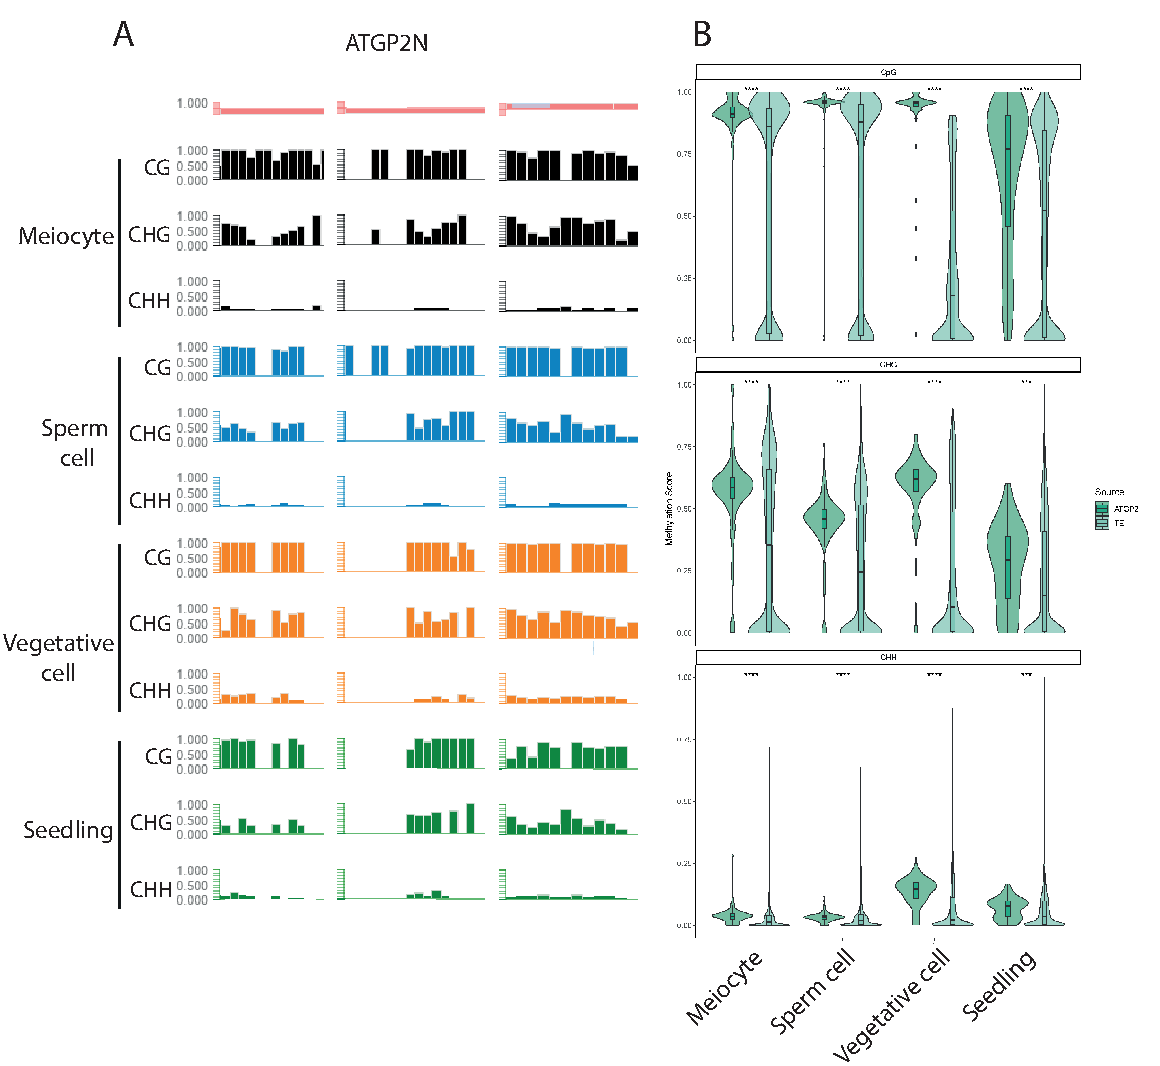
\includegraphics[width=1\textwidth]{Chapter2/Figs/Figure14_TE_methylation.pdf}
\caption{\textbf{ATGP2N TEs produce highly abundant 24nt sRNAs in the sperm cell, sperm nucleus and pollen}}
\label{fig:TE_methylation}
\captionsetup{font=small}
    \caption*{(A) Snapshot CHH methylation levels of three ATGP2N TEs which produces abundant sRNAs in the sperm. (A) Boxplots of CG, CHG and CHH methylation levels of the ATGP2 subset compared to all TEs in germline and somatic tissues. ***: p-value < 0.001, **: p-value < 0.01,*: p-value < 0.05}
\end{figure}

\clearpage

\section{Discussion}

\clearpage

\section{Materials and Methods}

\subsection{Plant materials and growth conditions}

\textit{Arabidopsis thaliana} plants were grown in 16h light/8h dark conditions, in 21°C, 70\% humidity in a controlled environment chamber on germination medium (GM) without glucose supplementation. The following lines have been grown: Col-0 wild type plant for the microspore and pollen sRNA sequencing libraries. For the anther imaging experiments, the transgenic reporter lines pCLSY1::CLSY1-eGFP (clsy1), pCLSY2::CLSY2-eGFP (WT), pCLSY3::-CLSY3-Venus (clsy3) and pCLSY4::CLSY4-eGFP (clsy4), pNRPD1::NRPD1-eGFP (WT), pNRPE1::NRPE1-eGFP (WT) were used with pAGO4::AGO4-Venus or ), pCLSY3::-CLSY3-Venus (clsy3) for a positive control.

\subsection{Microscopy}

Meiocyte and microspore stage anthers were dissected using a Leica dissecting microscope on 0.8\% agar and vacuum infiltrated in DAPI buffer (Galbraith’s buffer (45 mM MgCl2-6H2O, 30 mM trisodium citrate, 20 mM MOPS, pH 7.0), 1 µg/mL DAPI, and 0.01\% [v/v] Triton X-100) briefly, then imaged using imaging spacers (SecureSealTM Grace BioLabs). Individual microspores and pollen were imaged after isolation from unopened flower buds and opened flowers respectively, by collecting ~500 µL of flower buds into DAPI buffer, briefly vortexing and pelleting cells. All samples were imaged using Leica Stellaris 8 and Leica SP8X confocal microscopes.

\subsection{Isolation of microspores and pollen using fluorescence activated cell sorting}

\textit{Arabidopsis thaliana} microspores were isolated by manually collecting microspore stage flower buds, using the morphology described previously \citep{RN86}. The buds were collected into 1.5mL microcentrifuge tubes and suspended in PEB (10 mM CaCl2, 2 mM MES, 1 mM KCl, 1\% H3BO3, 10\% Sucrose, pH 7.5) buffer. The microspore cells were isolated as described previously \citep{RN140}. Briefly, the buds were gently ground in a clean pestle and mortar in PEB buffer and filtered through Miracloth (Merck-Millipore 475855) into a 1.5mL Eppendorf tube. This crude fraction was centrifuged for 5 minutes at 800g to gently pellet the microspore cells. The pellet was resuspended in 500µL PEB and sequentially filtered through 30µm and 20µm mesh filters (CellTrics®).

The fraction was separated using fluorescence-activated cell sorting (FACS) on a BD FACSMelody cell sorter (Beckton Dickinson) into TRI reagent (Zymo Research). The purity of the sorted cells was inspected using a widefield microscope.

Sperm cells were isolated as previously described \citep{RN140,RN141} except the sperm cell release step was repeated 4 times to maximise sperm cell release from pollen grain. Sperm cells were stained using SYBR green and SITOX orange and sperm cells and nuclei were sorted into TRI reagent (Zymo Research).

\subsection{sRNA sequencing}

RNA was released from isolated microspores by vortexing the samples with RNase free glass beads (Sigma-Aldrich) for 4 minutes before proceeding with RNA isolation. RNA was isolated from all samples using the Direct-zol™ RNA kit (Zymo Research, CN: R2061).

2 replicates of sRNA sequencing libraries were constructed per cell type (microspore, sperm cell, sperm nuclei) using the RealSeq®-biofluids NGS Library Preparation Kit for miRNAs and small RNAs. For the three library types the number of cells used for each replicate were as follows: 300 000 cells for microspore, 600 000 cells for sperm cells, and 1 500 000 cells for sperm nuclei.

Briefly, the RealSeq® adapters were ligated and blocked, then the sample was circularised, and the adapter dimers were removed. Then reverse transcription was performed as well as PCR amplification and size selection to end up with the final library.

Further, gel separation  and purification was performed to enrich the sRNA libraries for the desired fragment lengths (20-30 nucleotides long) as described previously \citep{RN187}. The libraries were ran on Novex TBE 6\% gels (Invitrogen, CN: EC6265BOX) along with a custom RNA ladder consisting of bands that were 146bp and 161bp in length. 

The gel was run for 45 mins with 120V and then stained using ethidium bromide. The gel was illuminated with UV light and the area between the two bands were then cut out using a clean razor blade and the gel slice was weighed. 2 volumes of elution buffer (0.5 M ammonium acetate, 10 mM magnesium sulfate, 1 mM EDTA (pH 8.0), 0.1\% SDS) was added to the gel slice. The sample was incubated at 37°C on a rotary platform (1000 RPM) for 4 hours. 

The sample was then centrifuged at 12000g for 1 minute at 4°C in a microcentrifuge. The supernatant was transferred into a fresh 1.5mL Eppendorf tube. An additional 200µL of elution buffer was added to the polyacrilamide gel fragment, vortexed, re-centrifuged and the two supernatants were combined. Any remaining fragments of polyacrilamide were removed  by passing the supernatant through a plastic column containng cellulose acetate filters. Two volumes of cold absolute ethanol was added and the solution was incubated on ice for 30 minutes. The DNA was recovered by centrifugation at 12000g got 10 minutes at 4°C. The pellet was dried and resuspended in 200µL TE buffer (10mM Tris-HCl, 1mM EDTA, pH 7.6) and 25µL of 3M sodium acetate (pH 5.2) was added. The precipitation step was repeated, the pellet was rinsed with 70\% ethanol and thoroughly dried before resuspending in TE buffer to a final volume of 30µL. The sample was incubated at 4°C overnight to redissolve the DNA.

The concentration and size distribution of purified sRNA libraries were determined using  High Sensitivity DNA Chips (Agilent Technologies, CN: 5067-5594).

The sRNA libraries were sequenced using a NextSeq 500 (Illumina).

\subsection{Bioinformatics and data analysis}

Adaptor trimming and filtering of reads that are 18nt to 28nt in length was performed on the raw sequencing data using Cutadapt \citep{RN88} v1.9.1). These reads were mapped to the Arabidopsis thaliana reference genome TAIR10 using Bowtie \citep{RN89}. 24nt clusters were extracted and loci were kept that overlapped previously determined non-overlapping genomic features of interest such as canocical RdDM loci (9629 loci), HyperTEs (797 loci), MetGenes (435 loci), transposons (TEs), genes17,20, and H3K9me2 enriched loci. These overlapping feature files were produced using BEDtools (v2.27.0) \citep{RN90}. 24nt sRNA clusters were extracted using ShortStack \citep{RN142} (n = 45639). To firstly identify true 24 nucleotide clusters, the ShortStack clusters from the two replicates were filtered to keep clusters where the predominant read length was 24 nucleotides long, where log2(RPKM+1) 24nt sRNA > log2(RPKM+1) 25nt sRNA +2 and that were >99bp (n = 34032).

Following this general filtering step, sperm cell specific clusters were identified where:
log2(RPKM+1) 24nt sperm cell sRNA > 0 \& where:
log2(RPKM+1) 24nt sperm cell sRNA - log2(RPKM+1) 24nt (other tissues: tapetum, meiocyte, microspore, root seedling and leaf) sRNA > 3 which resulted in 513 loci.

The euchromatic/heterochromatic annotation was allocated based on data from reference \cite{RN183} and classified into 5 chromatin states based on H3K9me2/H3: euchromatic (less than 0.6), intermediate euchromatic (bw. 0.6 and 0.9), intermediate (bw 0.9 and 1.4), intermediate heterochromatic (bw. 1.4 and 2.6), heterochromatic (above 2.6). 

The sRNA analysis pipeline is available from GitHub on request. Figures were plot using ggplot2 and pheatmap packages in R (v4.0.3).

